\documentclass[11pt]{article}
\pagestyle{plain}

\usepackage{graphicx}
\usepackage{amsmath}
\usepackage{amssymb}
%package pour les matrices

\pagestyle{plain}
\title{Rapport 3 : Algorithme QR}
\author{Loïc Jabiro KAYITAKIRE}
\date{NOMA : 53272100}

\begin{document}
\maketitle
\section{Théorie}

\subsection{Question 1}
Nous commencerons par prouver que si $A$ est normale, alors $A$ est diagonalisable.

Soit $A$ une matrice normale. Sa décomposition de Schur est :

$$A = UTU^*$$

avec $U$ une matrice unitaire et $T$ une matrice triangulaire supérieure.
Or, d'après la propriété des matrices normales :

$$AA^* = A^*A$$
$$(UTU^*) (UT^*U^*) = (UT^*U^*) (UTU^*)$$
$$UTT^*U^* = UT^*TU^*$$

En multipliant à gauche par $U^*$ et à droite par $U$, on obtient :

$$TT^* = T^*T$$

On a donc que $T$ est une matrice normale. Or, $T$ est triangulaire supérieure, et toute matrice normale triangulaire est diagonale. Donc, $T$ est diagonale. Donc, $A$ est semblable à une matrice diagonale, donc $A$ est diagonalisable.

Montrons maintenant que si $A$ est diagonalisable, alors $A$ est normale.

Soit $A$ une matrice diagonalisable. D'après la décomposition de Schur, on a $U$ unitaire et $T$ triangulaire supérieure tels que :
$$A = UTU^*$$

On a donc :

$$AA^* = (UTU^*) (UT^*U^*) = UTT^*U^*$$

et :

$$A^*A = (UTU^*)^*(UTU^*) = (UT^*U^*)(UTU^*) = UT^*TU^*$$

Or, $T$ est une matrice diagonale, donc $TT^* = T^*T$. On a donc que :
$$UTT^*U^* = UT^*TU^*$$ 
donc $AA^* = A^*A$. Donc, $A$ est normale.


\subsection{Question 2}
Si une matrice est Hermitienne ou symétrique, alors une moitié des informations contenues est redondante. On peut donc appliquer les calculs en utilisant qu'une moitié de la matrice.
Ensuite, comme la matrice est Hermitienne ou symétrique, la réduction à la forme de Hessenberg donne une matrice tridiagonale, augmentant grandement le nombre de valeurs nulles dans la matrice, et donc, réduisant le nombre d'opérations à effectuer.


\subsection{Question 3}
Soit la matrice $H_k$ suivante : 
$$H_k = \begin{pmatrix}
    a & b \\
    \epsilon & d \\
\end{pmatrix}$$

On va montrer, dans le cas réel, que pour $H_{k+1}$, l'élément sous-diagonal est en $O(\epsilon)$ lorsque l'on applique l'algorithme QR sans shifts.

Après une première itération de la méthode QR, on obtient :
$$Q = \begin{pmatrix}
    c & -s \\
    s & c \\
\end{pmatrix}$$
avec $c = \frac{a}{\sqrt{a^2 + \epsilon^2}}$ et $s = \frac{\epsilon}{\sqrt{a^2 + \epsilon^2}}$.
Et on a :
$$R = \begin{pmatrix}
    \sqrt{a^2 + \epsilon^2} & c b + s d \\
    0 & c d - s b \\
\end{pmatrix}$$

On obtient ainsi :
$$H_{k+1} = RQ = \frac{1}{a^2+\epsilon^2} \begin{pmatrix}
    a' & b' \\
    a d \epsilon - b \epsilon^2 & d' \\
\end{pmatrix}$$

On voit que l'élément sous-diagonal est en $O(\epsilon)$. On a donc une convergence linéaire de l'algorithme QR sans shifts.
\newline
Maintenant nous allons montrer que ce même élément est en $O(\epsilon^2)$ lorsque l'on applique l'algorithme QR avec le Rayleigh quotient shift.
On repart donc de la matrice $H_k$ et on applique la méthode QR avec shifts. On obtient donc en premier lieu :
$$H_k - \mu I = \begin{pmatrix}
    a - \mu & b \\
    \epsilon & d - \mu \\
\end{pmatrix}$$
Or, $\mu = d$, donc :
$$H_k - d I = \begin{pmatrix}
    a - d & b \\
    \epsilon & 0 \\
\end{pmatrix}$$
On applique ensuite la méthode QR et on obtient :
$$Q = \begin{pmatrix}
    c & -s \\
    s & c \\
\end{pmatrix}$$
avec $c = \frac{a - d}{\sqrt{(a - d)^2 + \epsilon^2}}$ et $s = \frac{\epsilon}{\sqrt{(a - d)^2 + \epsilon^2}}$.

$$R = \begin{pmatrix}
    \sqrt{(a - d)^2 + \epsilon^2} & c b \\
    0 & -s b \\
\end{pmatrix}$$

On obtient ainsi :
$$H_{k+1} = RQ + dI = \frac{1}{(a-d)^2+\epsilon^2} \begin{pmatrix}
    a' & b' \\
    - b \epsilon^2 & d' \\
\end{pmatrix}$$

On voit bien que l'élément sous-diagonal est en $O(\epsilon^2)$. On a donc bien une convergence quadratique de l'algorithme QR avec shifts.

\section{Rapport de performance}

\subsection{Complexité de l'algorithme QR}

D'après la théorie, l'algorithme QR utilisant la forme de Hessenberg a une complexité en $O(n^3)$, où $n$ est la taille de la matrice.

On voit sur le graphique ci-dessous que l'algorithme implémenté est relativement proche en complexité de celui de Scipy, qui sont tous deux en $O(n^3)$.

\begin{figure}[h]
\centering
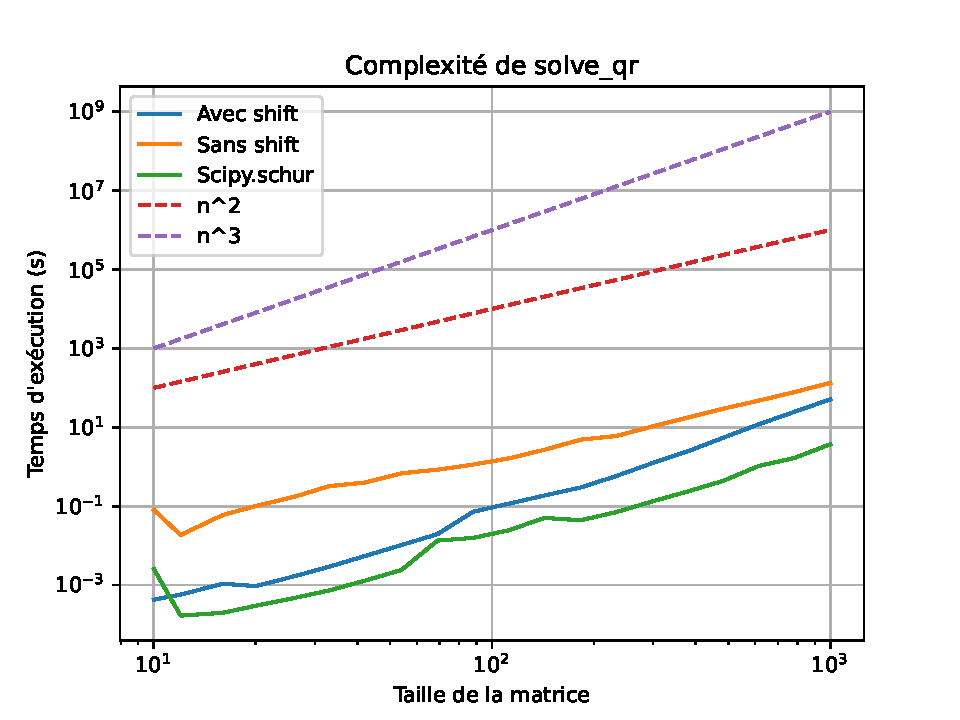
\includegraphics[width=0.8\textwidth]{images/compare_solve_qr_complexity.pdf}
\caption{Complexité de l'algorithme QR}
\end{figure}

On remarque tout de même que l'algorithme de Scipy est plus rapide que l'algorithme implémenté. Cela peut être dû à une meilleure gestion de la mémoire, ou à une meilleure implémentation de l'algorithme.
En particulier, le calcul de multiplication, peut être optimisé en utilisant l'algorithme de Strassen, qui a une complexité en $O(n^{2.81})$. 
On voit sur la figure ci-dessous que l'implémentation de Scipy est tout de même environ 10 fois plus rapide que mon implémentation.

\begin{figure}[h]
\centering
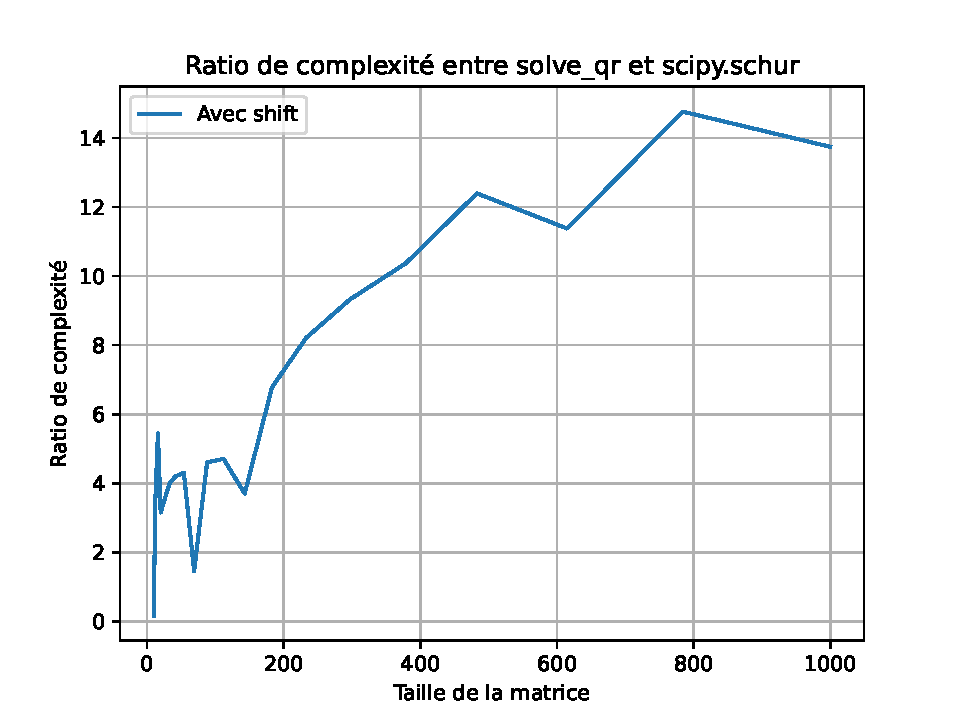
\includegraphics[width=0.8\textwidth]{images/compare_solve_qr_complexity_ratio.pdf}
\caption{Ratio entre les temps d'exécution de l'algorithme QR}
\end{figure}

\newpage

\subsection{Convergence de l'algorithme QR}
Nous avons montré plus haut que l'algorithme QR sans shifts a une convergence linéaire, tandis que l'algorithme QR avec shifts a une convergence quadratique.
Sur les graphiques ci-dessous, nous pouvons effectivement voir que l'algorithme QR avec shifts converge plus rapidement que l'algorithme QR sans shifts.

On voit également une convergence quadratique pour l'algorithme QR avec shifts, mais celui sans shifts atteint constamment le nombre maximal d'itérations.

\begin{figure}[h]
\centering
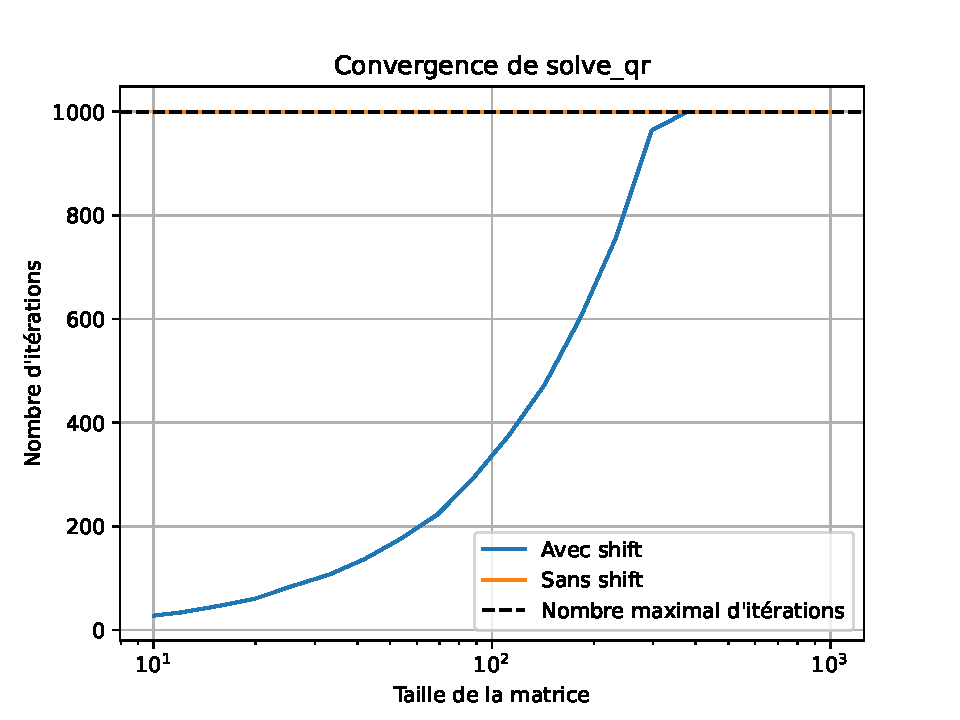
\includegraphics[width=0.8\textwidth]{images/compare_solve_qr_convergence_1000.pdf}
\caption{Convergence de l'algorithme QR (1000 itérations)}    
\end{figure}

\begin{figure}[h]
\centering
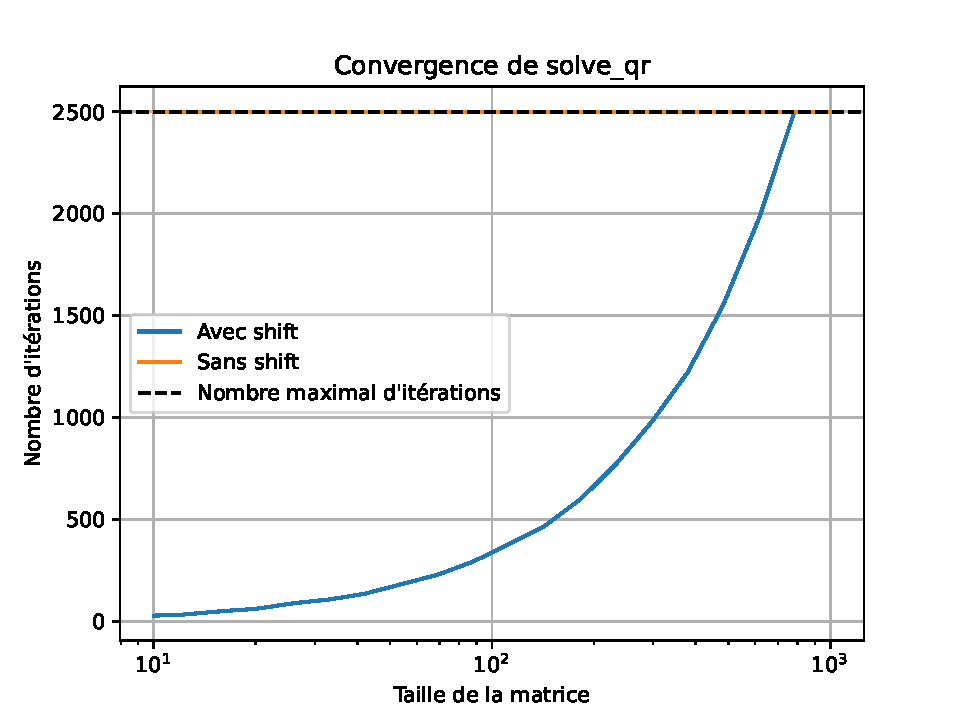
\includegraphics[width=0.8\textwidth]{images/compare_solve_qr_convergence_2500.pdf}
\caption{Convergence de l'algorithme QR (2500 itérations)}    
\end{figure}

\begin{figure}[h]
\centering
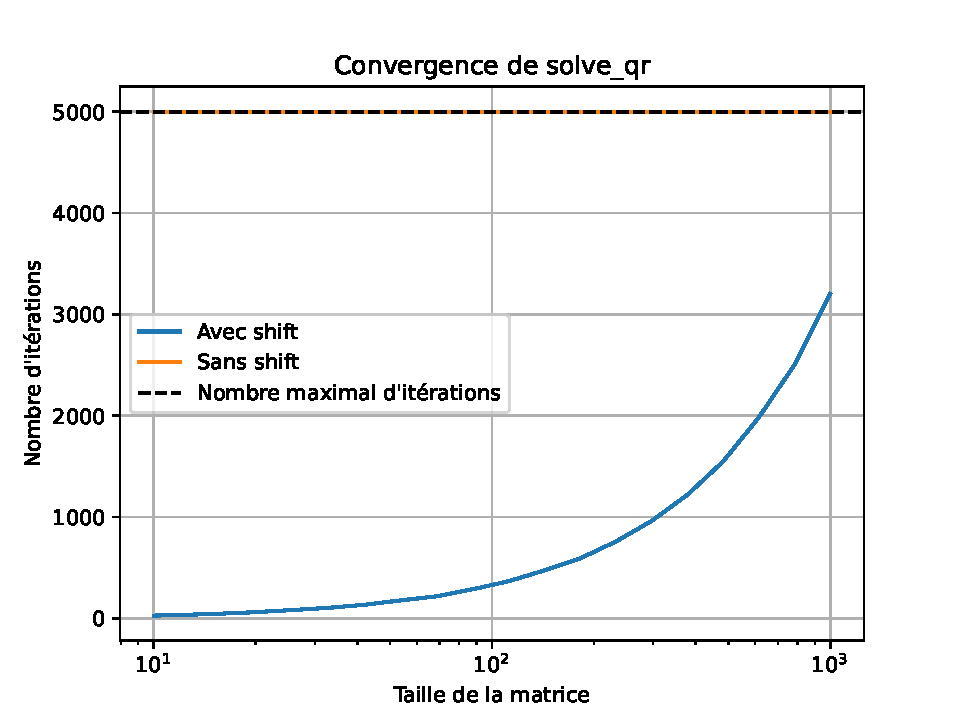
\includegraphics[width=0.8\textwidth]{images/compare_solve_qr_convergence_5000.pdf}
\caption{Convergence de l'algorithme QR (5000 itérations)}    
\end{figure}

\end{document}